\chapter{Introduction}

\section{Présentation de l'entreprise d'accueil}
Créée en 2003 par Laurent Py et Bruno LEGEARD, la société LEIROS est spécialisée dans le test logiciel. Elle est issue du projet Smart Testing\texttrademark ~au LIFC\footnote{Laboratoire d'informatique de Franche-Comté}. L'objectif premier de LEIROS a été d'industrialiser le projet Smart Testing\texttrademark.  LEIROS a ensuite changé de nom pour devenir SMARTESTING en juin 2008. En septembre 2008, Smartesting ouvre sa filiale à Bangalore, en Inde. SMARTESTING compte environ trente-cinq personnes dont onze dans le service R\&D{}\footnote{Recherche et développement}.

\subparagraph*{}
Smartesting est implantée dans différents points stratégiques. En France,le siège social ainsi que le centre R\&D sont à Besançon dans les locaux de l'hôtel d'entreprises TEMIS Innovation. Ainsi la R\&D reste proche géographiquement de l'université et de la recherche qui y a lieu. À Paris et à Amsterdam aux Pays-Bas se trouvent les agences où travaillent les commerciaux et les avant-vente. Smartesting s'est implantée à Bangalore, en Inde où elle compte réaliser la moitié de son chiffre d'affaires en 2010 grâce au boom de l'offshore où le marché du test logiciel est en pleine expansion.

%TODO : figure de temis innovation

\subparagraph*{}
Smartesting développe dans le secteur grandissant du test logiciel. Ce marché devrait atteindre 13 milliards de dollars en 2010 (selon une étude de Gartner). Le test logiciel, en particulier le test fonctionnel devient une phase clé du développement logiciel. Des besoins très stricts pour les milieux bancaires par exemple obligent ces entreprises à faire appel à des ingénieurs et des architectes de test afin de concevoir les tests logiciels qui permettront par exemple de garantir la stabilité, la non regression et le bon fonctionnement de gros projets. SMARTESTING propose Test Designer, une solution de génération automatique de référentiels de test à plusieurs niveaux.

\subparagraph*{}
L'entreprise est organisée autour d'un directoire de trois personnes : Laurent PY, Bruno LEGEARD et Stéphane WERBA.Je travaille dans le service de R\&D{}\ de SMARTESTING.  L'équipe est composée de 11 ingénieurs dévelopeurs qui améliorent sans cesse le produit Test Designer ainsi que les connecteurs et les publishers y sont développés. L'équipe fonctionne autour de méthodes Agiles, en particulier eXtreme Programming. Ces sujets seront développés dans les sections qui vont suivre.

\begin{figure}[!ht]
\centering
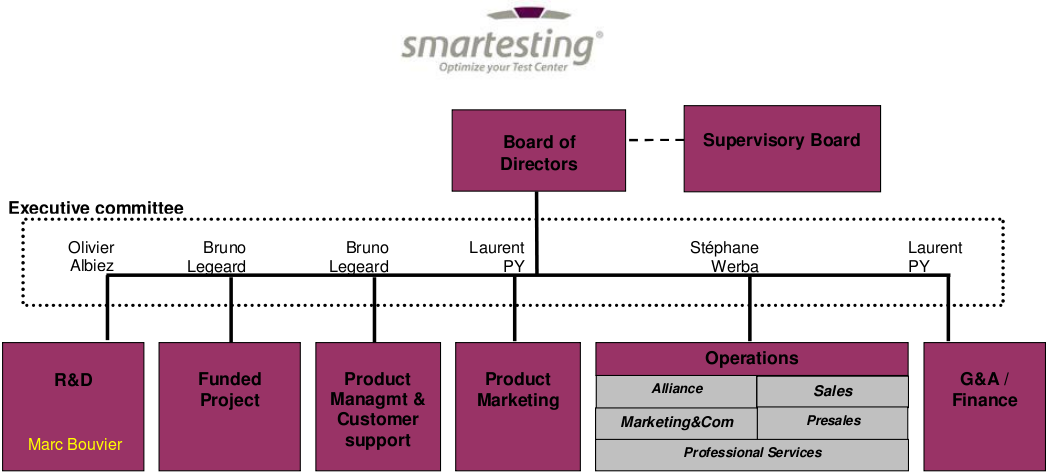
\includegraphics[width=\textwidth]{Illustrations/Organigramme_with_me.png}
\caption{Organigramme}
\label{figure:Organigramme de Smartesting}
\end{figure}

\section{Test Designer}
La solution Test Designer permet de générer des référentiels de tests fonctionnels à partir de modèles UML pour le test/footnote{Model Based Testing}. Elle fait le lien entre la modélisation de tests et le management de tests.

%Figure 
\begin{figure}[!ht]
\centering
\includegraphics[width=\textwidth]{Illustrations/TheSolutionSmartesting.png}
\caption{La solution SMARTESTING}
\label{figure:La Solution SMARTESTING}
\end{figure}



\subparagraph*{}
La modélisation de tests se fait à l'aide de modeleurs UML basés sur Eclipse\footnote{Eclipse est une plateforme applicative sur laquelle peuvent se greffer des applications clientes sous forme de plugins(extensions)}. Les modeleurs supportés actuellement par Test Designer sont Borland Together 2008 et IBM Rational Software Modeler 7.0.5 \& 7.5. 



%figure : Test Industrialization with Smartesting Center™

\section{Environnement de travail}
La première tâche qui m'a été confiée à mon arrivée fut d'installer mon poste de travail. Un ordinateur avec Ubuntu 8.10 m'a été confié et j'y ai installé IntelliJ Idea 8.0 (IDE\footnote{Environnement de développement intégré}), adapter quelques options de configuration au développement sur le projet Test Designer.

%%%%%%%%%%%%%%%%%%%%%%%%%%%%%%%%%%%%%%%%%%%%%%%%%%%%%%%%%%%%%%%%%%
%%%%%%%%%%%%%% Vieille version %%%%%%%%%%%%%%%%%%%%%%%%%%%%%%%%%%%
%%%%%%%%%%%%%%%%%%%%%%%%%%%%%%%%%%%%%%%%%%%%%%%%%%%%%%%%%%%%%%%%%%

%\chapter{Introduction}
%
%Il s'agit dans ce chapitre, de présenter la société Smartesting, son produit développé et, le contexte de travail dans lequel le stage de Master Professionnel Informatique option Systèmes Distribués et Réseaux de l'université de franche-comté a eu lieu.
%
%\section{Présentation de l'entreprise}
%
%Le stage s’est déroulé dans la société Smartesting située à Temis (figure \ref{Temis}) de Besançon. Il s'agit d'une société née il y a six ans à partir de travaux de recherches menés au LIFC\footnote{LIFC : Laboratoire d'Informatique de Franche-Comté} sur la génération de tests. 
%Ce sont Laurent Py et Bruno Legeard qui, en 2003, ont ainsi créé la société Leirios qui deviendra  Smartesting en juin 2008.
%Celle-ci emploie plus d'une trentaine de personnes dont dix en R\&D\footnote{R\&D : Recherche et développement} où mon stage a eu lieu.
%
%\begin{figure}[!ht]
%\begin{center}
%  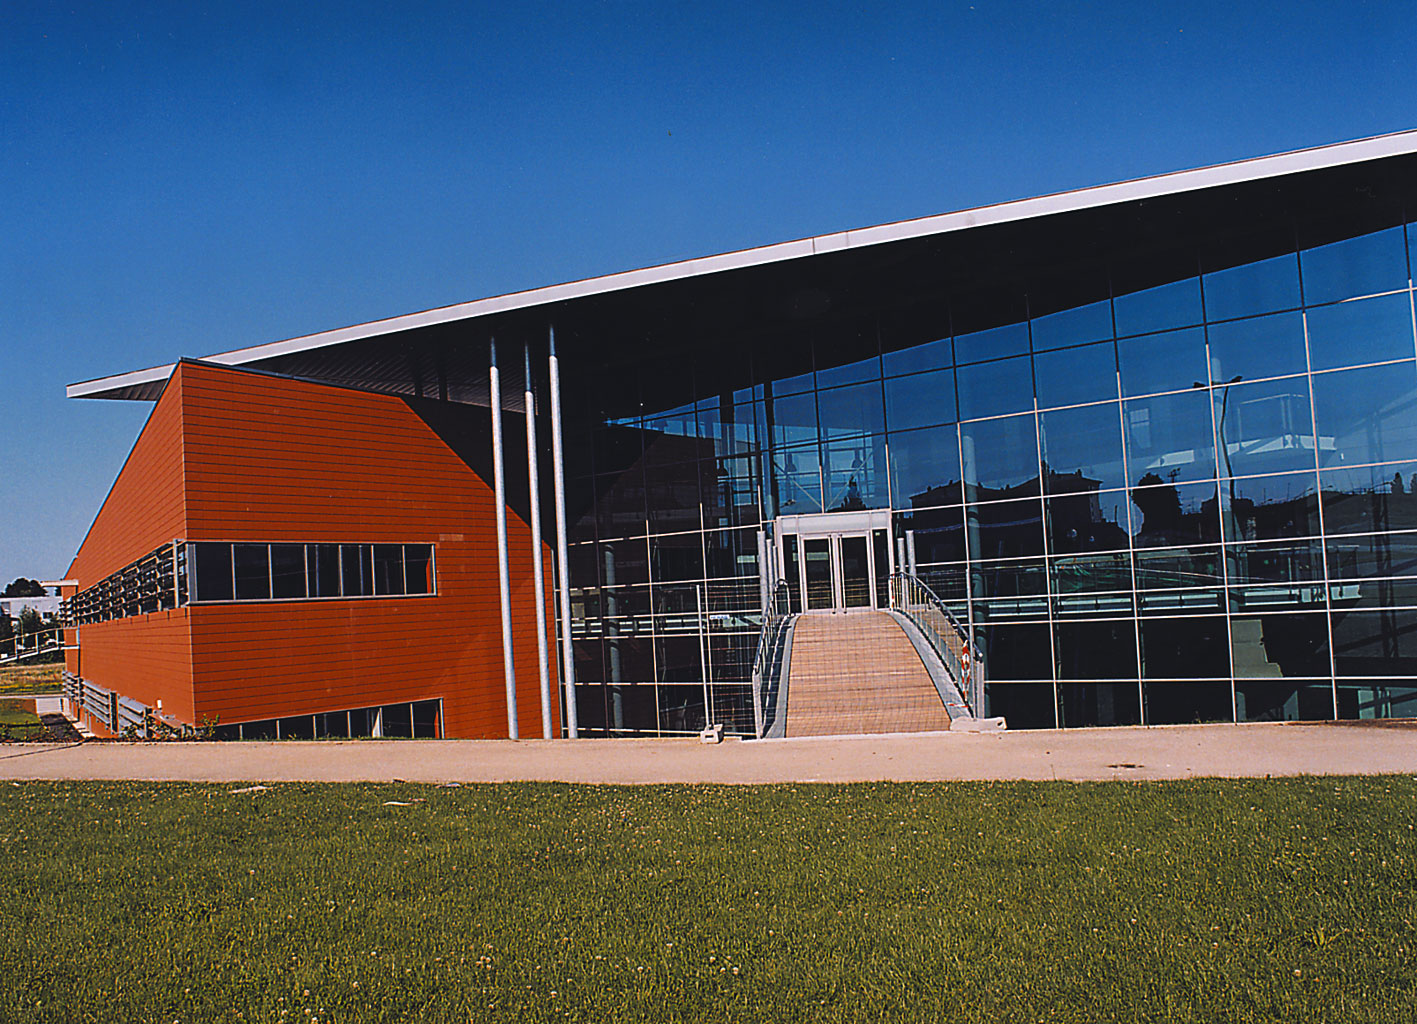
\includegraphics[height=5cm]{images/temis.jpg}
%  \caption{Temis innovation}
%  \label{Temis}
%\end{center}
%\end{figure}
%
%Smartesting est un éditeur de logiciel de génération automatique des cas de test à partir d'une modélisation UML des exigences. Smartesting utilise des outils de modélisation du marché basés sur Eclipse. Deux outils de modélisation sont supportés : IBM Rational Software Modeler\footnote{RSM ou équivalent comme IBM Rational Software Architect} et Borland Together. L'interface avec Smartesting se fait par l'intermédiaire d'un <<plug-in>> Eclipse spécifique à Smartesting (cf. figure \ref{SolutionSmartesting} p. \pageref{SolutionSmartesting}).
%
%\begin{figure}[!ht]
%\begin{center}
%  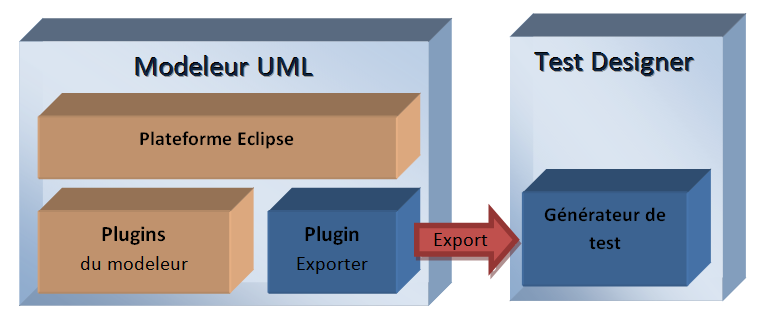
\includegraphics[width=.7\textwidth]{images/TestDesigner.png}
%  \caption{Solution Smartesting}
%  \label{SolutionSmartesting}
%\end{center}
%\end{figure}
%
%\subparagraph*{}
%La société est organisée en trois services distincts qui sont :
%\begin{itemize}
%  \item les commerciaux
%  \item les consultants
%  \item l'équipe R\&D
%\end{itemize}
% Durant le stage, j'ai rencontré l'ensemble des employés de Smartesting mais j'ai principalement travaillé avec la R\&D.
%
%\subparagraph*{}
%La R\&D où s'est déroulé mon stage, était un environnement de développement ``Agile''. 
%Il s'agit d'une méthode basée sur le développement itératif, où les exigences et les solutions évoluent grâce à la collaboration. 
%La gestion du projet avec les méthodes Agiles encourage les processus d'inspections et de remise en question de l'équipe de façon fréquente. 
%En générale, la philosophie des responsables est l'encouragement de l'équipe, l'auto-organisation et les responsabilités. 
%Ensemble qui pousse l'utilisation de bonnes pratiques de programmation et la mise en place de systèmes de livraison rapide, fiable et en adéquation avec les besoins clients et l'objectif de la société.
%Ceci étant obtenu grâce à un réseau de communication rapproché et un processus de fabrication sans gaspillage.
%
%\section{La solution Smartesting}
%
%De manière plus précise (cf. \ref{figure:TheSolutionSmartesting} p.\pageref{figure:TheSolutionSmartesting}), à partir des besoins métier et des exigences de test, est réalisé un modèle UML.
%Ce modèle peut être uniquement réalisé à partir des deux modeleurs RSM et Together.
%Il s'agit de modeleurs basés sur la plateforme Eclipse. Eclipse est une architecture de plugins qui communiquent les uns avec les autres pour former une application. C'est via ce mécanisme que Smartesting a développé deux plugins d'exportation de modèle pour les deux modeleurs précédemment cités.
%
%\subparagraph*{}
%Le logiciel ``Test Designer'' va quant à lui, générer des tests de manière automatique à partir du modèle exporté.
%Le résultat des tests est stocké dans un référentiel de test de Test Designer.
%Puis, ces tests vont être publiés dans un environnement de test tiers.
%
%\begin{figure}[!ht]
%\begin{center}
%  \includegraphics[width=\textwidth]{images/TheSolutionSmartesting.png}
%  \caption{La solution Smartesting complète}
%  \label{figure:TheSolutionSmartesting}
%\end{center}
%\end{figure}
%
%\subparagraph*{}
%Smartesting peut publier vers plusieurs environnements de gestion de tests. Ces environnements permettent par exemple de suivre l'évolution du test tout au long de son cycle de vie. Ensuite grâce à une couche d'adaptation, l'application modélisée pourra être testée.
%
%\subparagraph*{}
%Le processus de génération de tests de la solution Smartesting est un processus itératif. C'est à dire que si l'application déjà testée doit évoluée, la prise en compte des nouvelles fonctionnalités, ne générera pas un nouveau coût de génération des tests. 
%Il suffit de modifier le modèle UML de spécifications via le modeleur, puis de générer les tests à nouveau (automatique).
%
%\subparagraph*{}
%Traditionnellement la génération de tests est effectuée manuellement par un ingénieur de tests.
%
%\section{Objectifs}
%
%L’objectif de ce stage est d'intégrer un nouveau modeleur, mais cette fois open source, à l'ensemble des modeleurs compatibles avec la solution Smartesting.
%Et c'est à la suite du projet VETESS\footnote{VETESS : Vérification de systèmes embarqués VEhicules par génération automatique de TESts à partir des Spécifications}, dans lequel Smartesting est partenaire, que le choix du modeleur Papyrus a eu lieu.
%
%\subparagraph*{
\includegraphics[height=1cm]{images/logo-vetess.png} :}
%L’objectif stratégique du projet VETESS est de produire des outils conceptuels, méthodologiques et techniques pour la vérification de systèmes mécatroniques embarqués véhicule par génération automatique de tests à partir des spécifications de ces systèmes.
%
%
%\subparagraph*{}
%Pour remplir ces objectifs, le projet VETESS s’appuie sur un partenariat fortement complémentaire avec une expertise importante dans l’ingénierie dirigée par les modèles et la génération automatique de tests (figure \ref{figure:PartenairesVetess} p.\pageref{figure:PartenairesVetess}). 
%Il réunit un industriel soucieux de maîtriser la complexité des systèmes grand public (PSA Peugeot Citroën), à une PME innovante (Smartesting) leader dans le domaine du test à partir de modèle et, à un industriel Clemessy spécialisé possédant une offre de premier plan en matière de bancs de test de système électriques et électroniques embarqués. 
%Au niveau académique, les laboratoires impliqués (Université de Haute Alsace – Laboratoire MIPS et Université de Franche-Comté – Equipe LIFC) sont reconnus respectivement dans le domaine de la modélisation logicielle et système, et de la génération de tests.
%
%\begin{figure}[!ht]
%\begin{center}
%  
\includegraphics[width=\textwidth]{images/PartenaireVetess.png}
%  \caption{Partenaires VETESS}
%  \label{figure:PartenairesVetess}
%\end{center}
%\end{figure}
%
%\subparagraph{La solution Smartesting par rapport à VETESS :}
%Il est important que Smartesting puisse proposer sa solution aux entreprises qui souhaitent valider des systèmes embarqués.
%C'est pour cela qu'intégrer le modeleur choisit dans le projet VETESS est un atout commercial important pour Smartesting.
%Il s'agit d'offrir la possibilité a ses clients, d'utiliser le modeleur Papyrus comme modeleur de la solution.
%Sur la figure \ref{ObjectifPapyrus} p.\pageref{ObjectifPapyrus} l'objectif en image, propose trois plugins d'exportation de modèle.
%
%\begin{figure}[!ht]
%\begin{center}
%  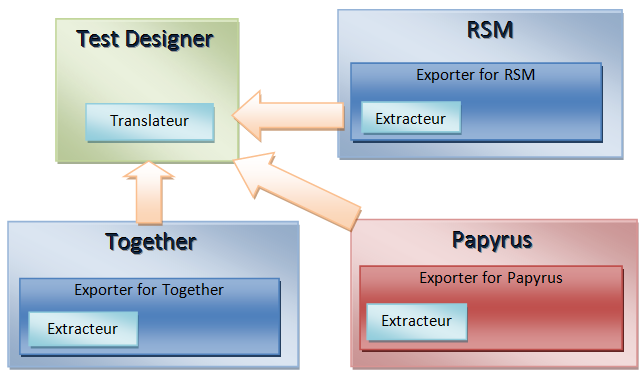
\includegraphics[height=5cm]{images/objectif_papyrus2.png}
%  \caption{Objectif : intégration du modeleur Papyrus}
%  \label{ObjectifPapyrus}
%\end{center}
%\end{figure}
%
%\subparagraph*{}
%A la différence de la figure \ref{ObjectifPapyrus} p.\pageref{ObjectifPapyrus}, il ne s'agit pas de recréer obligatoirement un plugin spécifique à Papyrus. 
%Il faut étudier le modeleur Papyrus afin de constater des éventuels points communs avec les modeleurs existants.
%C'est à partir de l'étude des points communs avec les autres modeleurs qu'il a été évoqué le besoin de fragmenter l'existant en plugins.
%
%\subparagraph{Fragmentation en plugins :}
%La fragmentation en plugins est un objectif secondaire. 
%Cela doit permettre la réorganisation des modules en plugins, afin de pouvoir utiliser du code commun.
%La ``pluginisation'' de l'application a posé quelques problèmes techniques.
%En particulier, la construction du produit appelé le \build a nécessité un gros chantier d'amélioration.
%
%\subparagraph*{}
%Le \build est un terme utilisé pour définir le processus automatisé qui permet de construire et déployer la solution Smartesting sur différentes plateformes telles que Linux et Windows, et sur différents modeleurs comme \together, \rsm et ``Papyrus''.
%Pour Smartesting, ce sont des tâches \textit{ant} qui réalisent l'automatisation du processus de construction du produit.
%
%L'amélioration du \build et la modification de l'infrastructure des modules doivent permettre d'atteindre le genre d'architecture de la figure \ref{reorganisation} (p.\pageref{reorganisation}).
%
%\begin{figure}[!h]
%\begin{center}
%  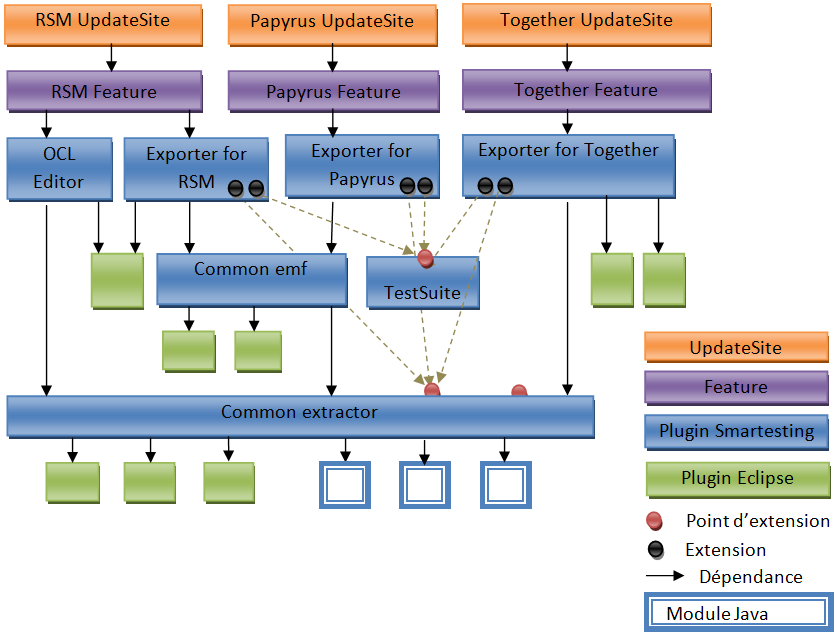
\includegraphics[width=\textwidth]{images/reorganisation2.png}
%  \caption{Réorganisation en plugins}
%  \label{reorganisation}
%\end{center}
%\end{figure}
%
%L'amélioration du \build doit permettre de créer les plugins mais aussi de les déployer. La figure \ref{reorganisation} montre les différents modules à déployer avec le \build :
%\begin{itemize}
%  \item Le plugin (en bleu)
%  \item La feature (en violet)
%  \item L'update site (en orange)
%\end{itemize}
%\ \\
%Ces trois types de modules permettent de déployer un plugin sur un modeleur type, grâce à un update-site.
%
%\subparagraph*{}
%La figure \ref{reorganisation} montre le travail complet de réorganisation de l'architecture de l'application. 
%En outre, l'utilisation des points d'extension a permis de faciliter l'intégration du spécifique dans les modeleurs.
%Grâce à ce mécanisme, il est possible d'adapter le comportement d'un plugin sans ajouter de dépendances entre le plugin standard et le plugin spécifique. 
%Exemple sur la figure \ref{reorganisation} p.\pageref{reorganisation} le plugin ``Exporter for RSM'' utilise le point d'extension du plugin ``Common extractor'' (point noir).
%En faisant cela, le plugin ``Common extractor'' (point rouge) est capable d'interroger le plugin ``Exporter for RSM'' afin qu'il réalise une extraction spécifique.
%Cela permet d'éviter de créer une dépendance au plugin spécifique \rsm. Ceci est aussi appelé une inversion de dépendance.
%
%\section{Méthode de travail}
%
%Le déroulement du stage s'est effectué au sein d'une équipe de développement ``Agile'' ou eXtrem Programming (XP).
%Cette méthode valorise la cohésion d'équipe et l'auto-organisation. 
%La fabrication de quelque chose doit toujours être réalisée sans contrainte, dans des conditions dites de ``fun'', terme extrait d'un livre dont le titre est <<Art of Agile development>>. 
%Il s'agit d'une lecture que j'ai faite durant le stage pour préparer les discussions collectives sur quelques chapitres. 
%
%\subparagraph*{}
%Dès le départ, ce qu’il faut comprendre de la méthode ``Agile'' est que le processus de développement peut être sans cesse amélioré. 
%Il y a quelques fois un groupe de lecture et chaque semaine une rétrospective qui donne lieu à des discussions. 
%Celles-ci permettent d’améliorer le processus de développement.
%C’est ainsi que j'ai pu participer à certains changements.
%
%La semaine est organisée en plusieurs événements répartis sur cette dernière et des réunions chaque midi appelées également morning meeting ou standup meeting.
%
%\subsection{Morning meeting}
%
%Chaque midi, l'équipe R\&D se réunit avant la pause pour faire le point sur le travail en cours de chacun. Tout le monde peut participer à cette réunion, pas seulement les membres de l'équipe R\&D. Cette réunion très courte permet de prendre connaissance du travail de ses collègues. Elle permet également de passer une annonce.
%
%\subparagraph*{}
%Ensuite, la semaine débute par une rétrospective, genre de bilan d’une semaine de travail, qui représente aussi en méthode XP une itération. 
%
%\subsection{Rétrospective}
%
%La rétrospective est une réunion qui dure environ une heure et qui permet de s’exprimer et d’évacuer les frustrations éventuelles ressenties lors de l’itération passée.
%Chaque semaine un animateur a pour rôle de faire participer tous les employés R\&D et de time boxer\footnote{Time boxé : Expression pour dire par exemple que l’on contrôle le temps de la réunion} la réunion. Les stagiaires ni sont pas exempts. 
%
%\subparagraph*{}
%Enfin, le travail de la semaine est planifié par le client XP à la fin de la rétrospective. Éventuellement, celui-ci peut demander une séance de cotation pour estimer le coût de développement d’une ou plusieurs fonctionnalités appelées aussi fiches blanches.
%
%\subsection{Séance de cotation}
%
%Le travail est organisé à partir de fiches représentant le travail à réaliser. Il peut s’agir d’une fonctionnalité à développer, d'un bug à corriger ou d'un travail d’exploration à effectuer.
%
%\subparagraph*{}
%Une fois les fiches cotées, le client XP peut proposer le travail à faire pour l’itération lors de l’engagement.
%
%\subsection{L'engagement}
%
%Le client XP dispose sur un tableau les fiches à réaliser par l’équipe de développement en fonction de l’effort que peut produire celle-ci. 
%Cet effort est un nombre de points définis par la R\&D. 
%Il s’agit de la vélocité, le client XP ne peut dépasser cette valeur.
%
%\subparagraph*{}
%Chez Smartesting, un point correspond au travail effectué durant une demi-journée sur une fiche sans interruption.
%
%\subsection{Pair Programming}
%
%Le ``Pair programming'' est une pratique qui consiste à réaliser une tâche par binôme. 
%Ce procédé permet une meilleure qualité du travail accompli, de prendre de meilleures décisions, d'aller plus vite que tout seul et surtout il permet d'éviter de rendre quelqu'un indispensable.
%
%\subparagraph*{}
%Le travail en paire a déjà été pratiqué à l'Université lors de projets.
%Mais cela prend une autre dimension en entreprise lorsque l'on travaille avec quelqu'un qui connaît bien son sujet et qui nous l'explique. 
%Très vite, on connaît le principe de fonctionnement de l'application et l'on peut commencer à participer aux cotations de fiches.
%
%\subsection{Batman et Robin}
%
%Le batman est le nom donné à la personne qui joue le rôle de superviseur de l'itération.
%Il est là pour surveiller le déroulement des fiches.
%Il discute avec les développeurs afin de vérifier ce qui va être réalisé ou ce qui est en cours de réalisation.
%
%\subparagraph*{}
%Il peut poser des questions au client XP à la place des développeurs.
%Il peut aussi demander au client XP d'aller voir les développeurs pour ré-expliquer ce qu'il attend.
%Avec le client XP, il peut préparer la démonstration pour la rétrospective de l’itération.
%
%\subparagraph*{}
%Il est associé au veilleur (Robin) qui aide certain binôme dans la réalisation de leur fiche.
%Le veilleur peut être amené à faire rencontrer des développeurs, car il a jugé que cela pourrait les aider à mieux avancer dans leur travail.
%
%\subparagraph*{}
%Au delà du côté humain de la méthode de travail ``Agile'', il y a toute l'infrastructure de développement du logiciel. Celle-ci permet de garantir la fiabilité et la non régression du logiciel développé.
%
%\subsection{Intégrateur continu}
%
%L'intégration continue est un élément essentiel gage de qualité fonctionnelle du programme développé.
%L'intégrateur est chargé d'exécuter en continu plusieurs tâches :
%\begin{itemize}
%  \item Les tests unitaires
%  \item Les tests fonctionnels (Test fit)
%  \item Les tests haut niveau (High level)
%  \item Les tests smokes
%\end{itemize}
%\ \\
%La durée de détection d'un bug varie suivant la tâche exécutée. Les tests sont répartis sur plusieurs ordinateurs pour être exécutés en parallèle.
%
%\subparagraph*{}
%Les tests unitaires sont les plus rapides à détecter les erreurs de bas niveau.
%Pour arriver jusqu'aux tests dit smoke qui permettent de vérifier que l'application déployée fonctionne correctement. 
%Exemple, ce test peut détecter un problème de déploiement de librairie ou l'utilisation d'une librairie non compatible avec tel ou tel modeleur. 
%
%\subparagraph*{}
%Pour avoir une plus grande réactivité, un panneau lumineux représentant les grandes catégories de test définies plus haut, a été installé pour visualiser plus rapidement un test en échec.
%Ensuite, c'est à chacun de s'autogèrer pour réparer au plus tôt le problème.
%
%\section{Synthèse}
%
%L'objectif du stage dans la société Smartesting est principalement l'intégration du modeleur open source papyrus dans la solution Smartesting.
%Il y a cependant un autre objectif secondaire, qui est la fragmentation de l'existant en plugins.
%Ces deux objectifs sont étroitement liés, puisque sans la fragmentation en plugin, il n'est pas possible de créer un nouveau plugin pour Papyrus sans duplication de code.
%On remarque aussi que la fragmentation en plugin a généré des problèmes sur la construction du produit Smartesting.
%
%\subparagraph*{}
%En fait, l'objectif principal et secondaire de ce stage, sont aussi des objectifs pour Smartesting.
%Grâce à la fragmentation par exemple, Smartesting se rapproche d'avantage d'une intégration complète dans Eclipse et donne la possibilité de développer d'autres plugins plus aisément.
%
%\subparagraph*{}
%Voyons maintenant dans le second chapitre, comment le modeleur Papyrus fonctionne et quelles améliorations ont permis la fragmentation en plugins.
